%!TEX root = ../../da.tex

\chapter{Graph Machine-Learning Potentials}
\label{ch:glps}


\begin{chapquote}{William Gibson, \textit{New Rose Hotel}}
    Not the Edge lecture again, I said.
    % Maas isn't like that, he said, ignoring me.\\
    % Maas was small, fast, ruthless. An atavism. Maas was all Edge.
\end{chapquote}

\marginnote[2\baselineskip]{We emphasise that such graph representations are not a novel concept. Graph kernels were proposed early to construct \ml models for molecules, for instance in reference~\cite{rps2007q} and references therein, and graph neural networks~\cite{bhlp2018m} have become a popular class of models for atomistic \ml. The aim of this section is to connect such graph-based \mlps to other \mlps and \ffs, arguing that they can be treated in a unified manner.}
\noindent
In this section, we discuss how interatomic potentials with a finite cutoff radius can be viewed as acting on a graph representation of a molecule or material. We introduce the term \glsfirst{glp}, or \newterm{graph potential}, to describe this class of interatomic potentials.
This class contains the \scare{bonded} terms of common \ffs, local \mlps, as well as models featuring message-passing mechanisms~\cite{gsvd2017q}, which allow semi-local interactions.

Having introduced this unified perspective, which specifies the \scare{forward} computation of the potential energy, we then argue that \ad affords a straightforward and efficient way to compute forces and stress tensors for \glps, even for periodic systems.
The definition of pairwise forces in many-body potentials is discussed briefly, and an overview and comparison of equivalent stress tensor formulations is provided.

\section{Semi-Local Interatomic Potentials}

\begin{figure*}
    \begin{tikzpicture}[
        x = 5.05cm,
        y = 3.5cm,
        >=stealth,
        ]
        \node (a) at (0,1.25) {
\begin{tikzpicture}[
    x = 0.8cm,
    y = 0.8cm,
    >=stealth,
    atom/.style = {circle, fill=black, minimum size=4pt,
    inner sep=0pt, outer sep=0pt},
    replica/.style = {circle, fill=red, minimum size=4pt,
    inner sep=0pt, outer sep=0pt, opacity=0.5},
]

\node[replica] (rep_0_00) at (0.0,0.0){};
    \node[replica] (rep_1_00) at (0.5,0.4){};
    \node[replica] (rep_2_00) at (1.2,0.5){};
    \node[replica] (rep_3_00) at (1.2,1.4){};
    \node[replica] (rep_4_00) at (1.7,1.0){};
    \draw [dashed] (0.0,0.0) -- (2.0,0.0);
    \draw [dashed] (0.0,0.0) -- (0.0,1.4);
    \node[replica] (rep_0_01) at (0.0,1.4){};
    \node[replica] (rep_1_01) at (0.5,1.7999999999999998){};
    \node[replica] (rep_2_01) at (1.2,1.9){};
    \node[replica] (rep_3_01) at (1.2,2.8){};
    \node[replica] (rep_4_01) at (1.7,2.4){};
    \draw [dashed] (0.0,1.4) -- (2.0,1.4);
    \draw [dashed] (0.0,1.4) -- (0.0,2.8);
    \node[replica] (rep_0_02) at (0.0,2.8){};
    \node[replica] (rep_1_02) at (0.5,3.1999999999999997){};
    \node[replica] (rep_2_02) at (1.2,3.3){};
    \node[replica] (rep_3_02) at (1.2,4.199999999999999){};
    \node[replica] (rep_4_02) at (1.7,3.8){};
    \draw [dashed] (0.0,2.8) -- (2.0,2.8);
    \draw [dashed] (0.0,2.8) -- (0.0,4.199999999999999);
    \node[replica] (rep_0_10) at (2.0,0.0){};
    \node[replica] (rep_1_10) at (2.5,0.4){};
    \node[replica] (rep_2_10) at (3.2,0.5){};
    \node[replica] (rep_3_10) at (3.2,1.4){};
    \node[replica] (rep_4_10) at (3.7,1.0){};
    \draw [dashed] (2.0,0.0) -- (4.0,0.0);
    \draw [dashed] (2.0,0.0) -- (2.0,1.4);
    \node[atom] (atom_0) at (2.0,1.4){};
    \node[atom] (atom_1) at (2.5,1.7999999999999998){};
    \node[atom] (atom_2) at (3.2,1.9){};
    \node[atom] (atom_3) at (3.2,2.8){};
    \node[atom] (atom_4) at (3.7,2.4){};
    \draw [dashed] (2.0,1.4) -- (4.0,1.4);
    \draw [dashed] (2.0,1.4) -- (2.0,2.8);
    \node[replica] (rep_0_12) at (2.0,2.8){};
    \node[replica] (rep_1_12) at (2.5,3.1999999999999997){};
    \node[replica] (rep_2_12) at (3.2,3.3){};
    \node[replica] (rep_3_12) at (3.2,4.199999999999999){};
    \node[replica] (rep_4_12) at (3.7,3.8){};
    \draw [dashed] (2.0,2.8) -- (4.0,2.8);
    \draw [dashed] (2.0,2.8) -- (2.0,4.199999999999999);
    \node[replica] (rep_0_20) at (4.0,0.0){};
    \node[replica] (rep_1_20) at (4.5,0.4){};
    \node[replica] (rep_2_20) at (5.2,0.5){};
    \node[replica] (rep_3_20) at (5.2,1.4){};
    \node[replica] (rep_4_20) at (5.7,1.0){};
    \draw [dashed] (4.0,0.0) -- (6.0,0.0);
    \draw [dashed] (4.0,0.0) -- (4.0,1.4);
    \node[replica] (rep_0_21) at (4.0,1.4){};
    \node[replica] (rep_1_21) at (4.5,1.7999999999999998){};
    \node[replica] (rep_2_21) at (5.2,1.9){};
    \node[replica] (rep_3_21) at (5.2,2.8){};
    \node[replica] (rep_4_21) at (5.7,2.4){};
    \draw [dashed] (4.0,1.4) -- (6.0,1.4);
    \draw [dashed] (4.0,1.4) -- (4.0,2.8);
    \node[replica] (rep_0_22) at (4.0,2.8){};
    \node[replica] (rep_1_22) at (4.5,3.1999999999999997){};
    \node[replica] (rep_2_22) at (5.2,3.3){};
    \node[replica] (rep_3_22) at (5.2,4.199999999999999){};
    \node[replica] (rep_4_22) at (5.7,3.8){};
    \draw [dashed] (4.0,2.8) -- (6.0,2.8);
    \draw [dashed] (4.0,2.8) -- (4.0,4.199999999999999);
    \draw [solid, very thick] (2.0,1.4) -- (4.0,1.4);
\draw [solid, very thick] (4.0,1.4) -- (4.0,2.8);
\draw [solid, very thick] (4.0,2.8) -- (2.0,2.8);
\draw [solid, very thick] (2.0,2.8) -- (2.0,1.4);
\draw [dashed] (6.0,0.0) -- (6.0,4.199999999999999);
\draw [dashed] (6.0,4.199999999999999) -- (0.0,4.199999999999999);


\end{tikzpicture}
};
        \node (b) at (2.25,1.25) {
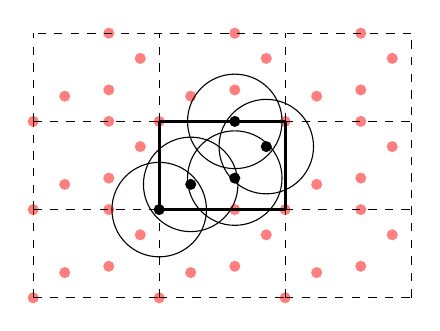
\begin{tikzpicture}[
    x = 0.8cm,
    y = 0.8cm,
    >=stealth,
    atom/.style = {circle, fill=black, minimum size=4pt,
    inner sep=0pt, outer sep=0pt},
    replica/.style = {circle, fill=red, minimum size=4pt,
    inner sep=0pt, outer sep=0pt, opacity=0.5},
]

\node[replica] (rep_0_00) at (0.0,0.0){};
    \node[replica] (rep_1_00) at (0.5,0.4){};
    \node[replica] (rep_2_00) at (1.2,0.5){};
    \node[replica] (rep_3_00) at (1.2,1.4){};
    \node[replica] (rep_4_00) at (1.7,1.0){};
    \draw [dashed] (0.0,0.0) -- (2.0,0.0);
    \draw [dashed] (0.0,0.0) -- (0.0,1.4);
    \node[replica] (rep_0_01) at (0.0,1.4){};
    \node[replica] (rep_1_01) at (0.5,1.7999999999999998){};
    \node[replica] (rep_2_01) at (1.2,1.9){};
    \node[replica] (rep_3_01) at (1.2,2.8){};
    \node[replica] (rep_4_01) at (1.7,2.4){};
    \draw [dashed] (0.0,1.4) -- (2.0,1.4);
    \draw [dashed] (0.0,1.4) -- (0.0,2.8);
    \node[replica] (rep_0_02) at (0.0,2.8){};
    \node[replica] (rep_1_02) at (0.5,3.1999999999999997){};
    \node[replica] (rep_2_02) at (1.2,3.3){};
    \node[replica] (rep_3_02) at (1.2,4.199999999999999){};
    \node[replica] (rep_4_02) at (1.7,3.8){};
    \draw [dashed] (0.0,2.8) -- (2.0,2.8);
    \draw [dashed] (0.0,2.8) -- (0.0,4.199999999999999);
    \node[replica] (rep_0_10) at (2.0,0.0){};
    \node[replica] (rep_1_10) at (2.5,0.4){};
    \node[replica] (rep_2_10) at (3.2,0.5){};
    \node[replica] (rep_3_10) at (3.2,1.4){};
    \node[replica] (rep_4_10) at (3.7,1.0){};
    \draw [dashed] (2.0,0.0) -- (4.0,0.0);
    \draw [dashed] (2.0,0.0) -- (2.0,1.4);
    \node[atom] (atom_0) at (2.0,1.4){};
    \node[atom] (atom_1) at (2.5,1.7999999999999998){};
    \node[atom] (atom_2) at (3.2,1.9){};
    \node[atom] (atom_3) at (3.2,2.8){};
    \node[atom] (atom_4) at (3.7,2.4){};
    \draw [dashed] (2.0,1.4) -- (4.0,1.4);
    \draw [dashed] (2.0,1.4) -- (2.0,2.8);
    \node[replica] (rep_0_12) at (2.0,2.8){};
    \node[replica] (rep_1_12) at (2.5,3.1999999999999997){};
    \node[replica] (rep_2_12) at (3.2,3.3){};
    \node[replica] (rep_3_12) at (3.2,4.199999999999999){};
    \node[replica] (rep_4_12) at (3.7,3.8){};
    \draw [dashed] (2.0,2.8) -- (4.0,2.8);
    \draw [dashed] (2.0,2.8) -- (2.0,4.199999999999999);
    \node[replica] (rep_0_20) at (4.0,0.0){};
    \node[replica] (rep_1_20) at (4.5,0.4){};
    \node[replica] (rep_2_20) at (5.2,0.5){};
    \node[replica] (rep_3_20) at (5.2,1.4){};
    \node[replica] (rep_4_20) at (5.7,1.0){};
    \draw [dashed] (4.0,0.0) -- (6.0,0.0);
    \draw [dashed] (4.0,0.0) -- (4.0,1.4);
    \node[replica] (rep_0_21) at (4.0,1.4){};
    \node[replica] (rep_1_21) at (4.5,1.7999999999999998){};
    \node[replica] (rep_2_21) at (5.2,1.9){};
    \node[replica] (rep_3_21) at (5.2,2.8){};
    \node[replica] (rep_4_21) at (5.7,2.4){};
    \draw [dashed] (4.0,1.4) -- (6.0,1.4);
    \draw [dashed] (4.0,1.4) -- (4.0,2.8);
    \node[replica] (rep_0_22) at (4.0,2.8){};
    \node[replica] (rep_1_22) at (4.5,3.1999999999999997){};
    \node[replica] (rep_2_22) at (5.2,3.3){};
    \node[replica] (rep_3_22) at (5.2,4.199999999999999){};
    \node[replica] (rep_4_22) at (5.7,3.8){};
    \draw [dashed] (4.0,2.8) -- (6.0,2.8);
    \draw [dashed] (4.0,2.8) -- (4.0,4.199999999999999);
    \draw [solid, very thick] (2.0,1.4) -- (4.0,1.4);
\draw [solid, very thick] (4.0,1.4) -- (4.0,2.8);
\draw [solid, very thick] (4.0,2.8) -- (2.0,2.8);
\draw [solid, very thick] (2.0,2.8) -- (2.0,1.4);
\draw [dashed] (6.0,0.0) -- (6.0,4.199999999999999);
\draw [dashed] (6.0,4.199999999999999) -- (0.0,4.199999999999999);


\draw (atom_0) circle (0.6cm);
\draw (atom_1) circle (0.6cm);
\draw (atom_2) circle (0.6cm);
\draw (atom_3) circle (0.6cm);
\draw (atom_4) circle (0.6cm);
\end{tikzpicture}
};
        \node (c) at (2.25,0) {
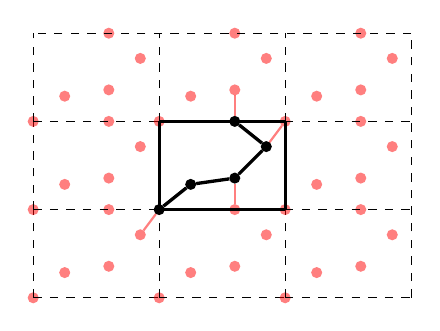
\begin{tikzpicture}[
    x = 0.8cm,
    y = 0.8cm,
    >=stealth,
    atom/.style = {circle, fill=black, minimum size=4pt,
    inner sep=0pt, outer sep=0pt},
    replica/.style = {circle, fill=red, minimum size=4pt,
    inner sep=0pt, outer sep=0pt, opacity=0.5},
]

\node[replica] (rep_0_00) at (0.0,0.0){};
    \node[replica] (rep_1_00) at (0.5,0.4){};
    \node[replica] (rep_2_00) at (1.2,0.5){};
    \node[replica] (rep_3_00) at (1.2,1.4){};
    \node[replica] (rep_4_00) at (1.7,1.0){};
    \draw [dashed] (0.0,0.0) -- (2.0,0.0);
    \draw [dashed] (0.0,0.0) -- (0.0,1.4);
    \node[replica] (rep_0_01) at (0.0,1.4){};
    \node[replica] (rep_1_01) at (0.5,1.7999999999999998){};
    \node[replica] (rep_2_01) at (1.2,1.9){};
    \node[replica] (rep_3_01) at (1.2,2.8){};
    \node[replica] (rep_4_01) at (1.7,2.4){};
    \draw [dashed] (0.0,1.4) -- (2.0,1.4);
    \draw [dashed] (0.0,1.4) -- (0.0,2.8);
    \node[replica] (rep_0_02) at (0.0,2.8){};
    \node[replica] (rep_1_02) at (0.5,3.1999999999999997){};
    \node[replica] (rep_2_02) at (1.2,3.3){};
    \node[replica] (rep_3_02) at (1.2,4.199999999999999){};
    \node[replica] (rep_4_02) at (1.7,3.8){};
    \draw [dashed] (0.0,2.8) -- (2.0,2.8);
    \draw [dashed] (0.0,2.8) -- (0.0,4.199999999999999);
    \node[replica] (rep_0_10) at (2.0,0.0){};
    \node[replica] (rep_1_10) at (2.5,0.4){};
    \node[replica] (rep_2_10) at (3.2,0.5){};
    \node[replica] (rep_3_10) at (3.2,1.4){};
    \node[replica] (rep_4_10) at (3.7,1.0){};
    \draw [dashed] (2.0,0.0) -- (4.0,0.0);
    \draw [dashed] (2.0,0.0) -- (2.0,1.4);
    \node[atom] (atom_0) at (2.0,1.4){};
    \node[atom] (atom_1) at (2.5,1.7999999999999998){};
    \node[atom] (atom_2) at (3.2,1.9){};
    \node[atom] (atom_3) at (3.2,2.8){};
    \node[atom] (atom_4) at (3.7,2.4){};
    \draw [dashed] (2.0,1.4) -- (4.0,1.4);
    \draw [dashed] (2.0,1.4) -- (2.0,2.8);
    \node[replica] (rep_0_12) at (2.0,2.8){};
    \node[replica] (rep_1_12) at (2.5,3.1999999999999997){};
    \node[replica] (rep_2_12) at (3.2,3.3){};
    \node[replica] (rep_3_12) at (3.2,4.199999999999999){};
    \node[replica] (rep_4_12) at (3.7,3.8){};
    \draw [dashed] (2.0,2.8) -- (4.0,2.8);
    \draw [dashed] (2.0,2.8) -- (2.0,4.199999999999999);
    \node[replica] (rep_0_20) at (4.0,0.0){};
    \node[replica] (rep_1_20) at (4.5,0.4){};
    \node[replica] (rep_2_20) at (5.2,0.5){};
    \node[replica] (rep_3_20) at (5.2,1.4){};
    \node[replica] (rep_4_20) at (5.7,1.0){};
    \draw [dashed] (4.0,0.0) -- (6.0,0.0);
    \draw [dashed] (4.0,0.0) -- (4.0,1.4);
    \node[replica] (rep_0_21) at (4.0,1.4){};
    \node[replica] (rep_1_21) at (4.5,1.7999999999999998){};
    \node[replica] (rep_2_21) at (5.2,1.9){};
    \node[replica] (rep_3_21) at (5.2,2.8){};
    \node[replica] (rep_4_21) at (5.7,2.4){};
    \draw [dashed] (4.0,1.4) -- (6.0,1.4);
    \draw [dashed] (4.0,1.4) -- (4.0,2.8);
    \node[replica] (rep_0_22) at (4.0,2.8){};
    \node[replica] (rep_1_22) at (4.5,3.1999999999999997){};
    \node[replica] (rep_2_22) at (5.2,3.3){};
    \node[replica] (rep_3_22) at (5.2,4.199999999999999){};
    \node[replica] (rep_4_22) at (5.7,3.8){};
    \draw [dashed] (4.0,2.8) -- (6.0,2.8);
    \draw [dashed] (4.0,2.8) -- (4.0,4.199999999999999);
    \draw [solid, very thick] (2.0,1.4) -- (4.0,1.4);
\draw [solid, very thick] (4.0,1.4) -- (4.0,2.8);
\draw [solid, very thick] (4.0,2.8) -- (2.0,2.8);
\draw [solid, very thick] (2.0,2.8) -- (2.0,1.4);
\draw [dashed] (6.0,0.0) -- (6.0,4.199999999999999);
\draw [dashed] (6.0,4.199999999999999) -- (0.0,4.199999999999999);

\draw [red, solid, opacity=0.5, thick] (rep_4_00) -- (atom_0);
\draw [solid, very thick] (atom_0) -- (atom_1);
% \draw [red, solid, opacity=0.5, thick] (atom_1) -- (rep_3_10);
\draw [solid, very thick] (atom_1) -- (atom_2);
\draw [solid, very thick] (atom_2) -- (atom_4);
\draw [red, solid, opacity=0.5, thick] (atom_2) -- (rep_3_10);
\draw [solid, very thick] (atom_3) -- (atom_4);
\draw [red, solid, opacity=0.5, thick] (atom_3) -- (rep_2_12);
\draw [red, solid, opacity=0.5, thick] (atom_4) -- (rep_0_22);

\end{tikzpicture}
};
        \node (d) at (0,0) {
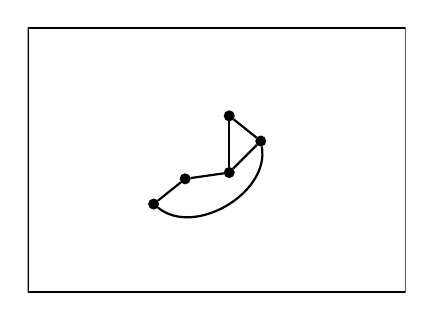
\begin{tikzpicture}[
    x = 0.8cm,
    y = 0.8cm,
    >=stealth,
    atom/.style = {circle, fill=black, minimum size=4pt,
    inner sep=0pt, outer sep=0pt},
    replica/.style = {circle, fill=red, minimum size=4pt,
    inner sep=0pt, outer sep=0pt, opacity=0.5},
]

\clip (0.0,0.0) rectangle (6.0,4.199999999999999);

\node[atom] (atom_0) at (2.0,1.4){};
\node[atom] (atom_1) at (2.5,1.7999999999999998){};
\node[atom] (atom_2) at (3.2,1.9){};
\node[atom] (atom_3) at (3.2,2.8){};
\node[atom] (atom_4) at (3.7,2.4){};
\draw [solid, thick] (atom_0) to [bend right=70] node [midway, above]{} (atom_4);
\draw [solid, thick] (atom_0) -- (atom_1);
\draw [solid, thick] (atom_1) -- (atom_2);
% \draw [solid, thick] (atom_1) -- (atom_3);
\draw [solid, thick] (atom_2) -- (atom_4);
\draw [solid, thick] (atom_2) -- (atom_3);
\draw [solid, thick] (atom_3) -- (atom_4);

\draw [solid, thick] (0.0,0.0) rectangle (6.0,4.199999999999999);


\end{tikzpicture}
};
        \draw [->] (a) to node [midway, above]{Determine neighbours} node [midway, below]{ $|\Rm_{ij}| < r_{\text{c}}$} (b) ;
        \draw [->] (b) -- (c) ;
        \draw [->] (c) to node [midway, above]{Construct graph} (d) ;
    \end{tikzpicture}
    \caption{Construction of a graph representation.}
    \label{fig:glp-sketch_graph}
\end{figure*}

The starting point for our considerations is an additive ansatz for the potential energy $U$, which we encountered in \cref{sec:ffs}.
In such interatomic potentials, $U$ is computed as the sum of atomic contributions $U_i$, which are in turn computed based on local neighbourhoods $\nbh{i}$ for each atom.
Due to the requirement of translational invariance, these contributions can only depend on atom-pair vectors; absolute positions cannot be used.\footnote{More precisely, it is advantageous to include translational symmetry when constructing models of the \bo \pes; see \cref{ssec:repsb_invariance}.}

Atomic potential energies therefore depend on pairwise connections to neighbouring atoms -- a description that can be formalised in terms of a graph, which we will now undertake.
% Continuing from \cref{sec:ml-mlps}, we consider \mlps of the form\marginnote[\baselineskip]{In this part of the thesis, we focus on periodic systems and therefore use $\Rsc$; the non-periodic case can be recovered by settings $\Basis$ larger than any possible interaction distance. We will also drop $\Charges$ from now on.}
% \begin{equation}
%   U(\Rsc, \Charges, \Basis) = \sum_{i \in \Rsc} U_i(\nhb{i}) \, ,
% \end{equation}
% where $\nbh{i} = \curlyset{j}{\magnitude{\Rm_{ij}} \leq \cutoff, j \in \Rsc}$.
% As discussed in \cref{ch:pbc}, in order to avoid discontinuities, we additionally require that $\cutoff$ is chosen such that at most one replica is within a given atomic environment.\footnote{In a general triclinic system, this means that $\cutoff \leq \min_{\alpha = 1, 2, 3} \recipn_\alpha \cdot \basis_\alpha$ with $\basis_\alpha$ denoting a lattice vector and $\recipn_\alpha$ the corresponding normalised reciprocal lattice vector; see \cref{ch:pbc}.}
\marginnote{In this chapter, we focus on periodic systems and therefore use $\Rsc$; the non-periodic case can be recovered by setting $\Basis$ larger than any possible interaction distance. We will also drop $\Charges$ from now on. In general additional labels can be assigned to nodes and edges, for instance for the purposes of message passing; we suppress such complications for now.
% Also note that nodes and edges may be associated with additional properties, such as atomic charges, bond information, or state vectors for the purposes of message-passing. For the present derivation, which is concerned with the system geometry encoded in $\graph$, this is not relevant, and will therefore be suppressed in the notation.
}
The foundation of graph potentials is a representation of the system under consideration as a directed graph $\graph = (\vertices, \edges)$, with the vertices (or nodes) $\vertices$ representing the atoms in the simulation cell, labeled by $Z_i$. The edges $\edges$ encode atomic neighbourhoods
\begin{align}
    \edges &= \curlyset{\Rm_{ij}}{\magnitude{\Rm_{ij}} \leq \cutoff,\, i,j \in \Rsc} \\
           &= \curlyset{\Rm_{ij}}{i \in \Rsc,\, j \in \nbh{i}} \, .
\end{align}
Crucially, as we rely on the \gls{mic} to construct $\graph$, it is boundary invariant.
As discussed in \cref{ch:pbc}, in order to avoid discontinuities, we additionally require that $\cutoff$ is chosen such that at most one replica is within a given atomic environment.\footnote[][2\baselineskip]{In other words, $\cutoff{<}\maxcutoff$ as defined in \cref{eq:pbc_maxcutoff}.} 
As opposed to the original definition of crystal graphs by Xie and Grossman~\cite{xg2018Aq}, $\graph$ therefore only contains single edges between vertices.\footnote{More precisely, each edge between vertices exists exactly twice, once in each direction. From a physical perspective, this definition amounts to a kind of \scare{double counting}, since $\R_{ij}=-\R_{ji}$; no information is added by taking both directions into account. However, this convention avoids the difficulty of defining an arbitrary ordering of edges, and can be used to distinguish derivatives at a later stage. We will make use of this in \cref{sec:hf_glps}.}
This construction is sketched in \cref{fig:glp-sketch_graph}.
We note in passing that the topology of $\graph$ can change during the course of an \md simulation; \glps must therefore be constructed to remain continuously differentiable as such changes occur.

\newthought{If we restrict interactions} to nearest neighbours on the graph, setting $U_i = U_i(\nbh{i})$, we recover the notion of a strictly local potential, and can therefore naturally describe any potential of this type, either \mlps or \ffs.
As the number of neighbours can be expected to remain constant as $N$ increases, provided we keep the density fixed as we take the limit, this yields $\bigo{N}$ scaling of energy predictions.
However, not all interactions of interest may be captured within $\cutoff$.

Let us therefore consider how to construct interactions beyond the cutoff. The simplest way would be to increase the cutoff radius directly, simply enlarging atomic neighbourhoods. This leads to a cubic increase in the size of neighbourhoods, which can introduce computational difficulties.\footnote{We note in passing that in the case of simple pairwise interactions, Ewald summation~\cite{e1921p,dyp1993p} or fast multipole methods~\cite{gr1987p,wh1994p} can be used to recover $\bigo{N \log N}$ or linear scaling, respectively. However, we consider general many-body interactions, where such techniques are not available at this point.}
Semi-local \glps{}~\cite{gsvd2017q,sktm2017q,sstm2018q,um2019q,kgg2020q,kbg2021q,ucsm2021q,bmsk2022q,bkoc2022q,bbkc2022a,blcd2022q} are an intriguing alternative construction. In such systems, longer-range interactions are iteratively built up from local ones by repeated interactions between neighbouring atomic environments. For $\interactions$ such interactions, the maximum effective cutoff radius therefore becomes $\effcutoff{\defas}\cutoff \interactions$, retaining most of the computational advantages of the original cutoff radius while allowing interactions beyond local neighbourhoods.
Alternatively, this approach can be viewed as an explicit sparsification of the full model within the extended neighbourhood defined by $\effcutoff$.
% , only allowing nearby atoms to interact directly.

% consider: (TF) Maybe mention that each interaction step between neighbourhoods is a mean field interaction which actually comes along with a loss of information (this can also leads to oversquashing kind of restricting the distance over which information can be propagated).

The \newterm{interaction order} $\interactions$ allows us to classify \glps. 
At $\interactions{=}1$, only information from direct neighbours of $i$ is used to compute $U_i$, at $\interactions{=}2$, the neighbours of all neighbours of $i$ are included as well, and so on.
In other words, $\interactions$ counts the maximum number of edges traversed from $i$ to compute $U_i$.
We introduce $\edgest{i}$ as that set of edges, and $\nbht{i}$ as the corresponding set of neighbourhoods.

\marginnote[1\baselineskip]{Note that while atomic potential energies have a range of $\effcutoff$, i.e., change only due to position changes within that radius, the forces can be influenced by changes up to $2\effcutoff$.}
For $\interactions{>}1$, the energy at an atom $i$ may depend on edges between atoms outside the local atomic neighbourhood. For this reason, we use the term \newterm{semi-local} \mlp, distinguishing from potentials with fully local character. 
However, we must emphasise that for finite $\interactions$, such models are still local\footnote{Non-local models are discussed briefly in \cref{part:end}.} in the extended neighbourhood within the cutoff radius $\effcutoff$. In order to realise the computational advantage associated with the smaller $\cutoff$, however, we cannot explicitly construct these extended neighbourhoods for each $i$.

\newthought{We finally define graph potentials} as potential energy functions where $U = 
\sum_{i \in \Rsc}\nolimits U_i(\graph)$. For this thesis, we further restrict \glps to those where $\effcutoff$ admits only interactions with single replicas.\footnote{This is not a crucial restriction, but it simplifies the comparison of heat flux formulations in \cref{ch:gk-hf}: If $\effcutoff{>}\maxcutoff$, the \gls{mic} does not apply and $\Jgmic$ is no longer equivalent to $\Junf$.}\footnote{This criterion is $\effcutoff{<}\maxcutoff$ as defined in \cref{eq:pbc_maxcutoff}.}
Setting $\interactions{=}1$, this definition includes distance-truncated terms of classical \ffs (see \cref{sec:ffs}), as well as \mlps that are not explicitly defined as graph \nns, provided that atomic potential energies are computed based on atom-pair vectors.

In this framework, as we rely on a cutoff radius to define $\graph$, we cannot readily describe potentials with global interactions or long-range electrostatics.
In some cases, for instance when inputs to electrostatics are predicted based on local environments~\cite{msb2012q,b2021q}, some of the present considerations could be nevertheless applied. We do not pursue this here.

\section{Message-Passing Neural Networks}

\marginnote[3\baselineskip]{To simplify the notation, we now drop the \mic label from $\Rm_{ij}$, as all $\R_{ij}$ appearing in the remainder of this section are edges in $\graph$ and therefore generated with the \mic in mind.}
Having introduced the abstract notion of semi-local \glps, we now consider their explicit construction using the 
\glsfirst{mpnn} architecture~\cite{gsvd2017q}. 
\mpnns operate on $\graph$ in three stages, illustrated in \cref{fig:glp-mpnn_sketch}: initialisation, message-passing, and readout, where each message-passing step is labeled by $t{=}0, \ldots, \interactions$. During initialisation ($t{=}0$), every atom $i$ is assigned a state vector $\state{i}{t=0}$, based on its chemical species. 
During the next stage, these states are \newterm{updated} with \newterm{messages} $\msg{i}{t}$ that can depend on the states of both the receiver atom $i$ and its neighbours $j \in \nbh{i}$, as well as on the edges $\R_{ij}$ connecting them:
%
\begin{align}
    \msg{i}{t+1} &= \sum_{j \in N(i)} \msgf{t}(\state{i}{t}, \state{j}{t}, \edge{i}{j}) \\
    \state{i}{t+1} &= \updatef{t}(\state{i}{t}, \msg{i}{t+1}) \, .
\end{align}
%
Here, the message functions\footnote[][-7\baselineskip]{In practice, message functions are not entirely arbitrary. To ensure smoothness, or more precisely, to ensure that the potential is a continuously differentiable function of positions, the message function typically incorporates a predefined cutoff function $\fcutoff(r_{ij})$. This function is defined such that contributions to energies and forces continuously approach zero as $r_{ij}$ approaches the cutoff radius $\cutoff$. If this is not the case, the resulting \ff ceases to be conservative and energy conservation is violated.} $\msgf{t}$ and update functions $\updatef{t}$ are differentiable functions implemented as neural networks. They are learned during training, and can differ over message-passing iterations.
The message functions $\msgf{t}$ model pairwise interactions. Their aggregation into the total message $\msg{i}{t+1}$ via a sum ensures permutational invariance.
The update functions $\updatef{t}$ describe how the interactions with all neighbours influence the new state of the receiver atom. Over multiple iterations, information is \emph{propagated} through the graph.
% up to $\interactions$ hops on the graph, or equivalently a distance of $\effcutoff$.

\begin{figure*}
    \begin{tikzpicture}[
        x = 6.5cm,
        y = 3.0cm,
        >=stealth,
        ]
        \node (a) at (0,1) {
\begin{tikzpicture}[
    scale=0.9,
    x = 0.8cm,
    y = 0.8cm,
    >=stealth,
    atom/.style = {circle, fill=black, minimum size=6pt,
              inner sep=0pt, outer sep=0pt},
    ]

\node[atom] (atom_0) at (1.0,1.5){};

\node[atom] (atom_1) at (2.0,1.5){};

\node[atom] (atom_2) at (3.0,1.5){};

\node[atom] (atom_3) at (4.0,1.5){};

\node[atom] (atom_4) at (5.0,1.5){};

\draw [->, solid, very thick, color=extra_0] (atom_0) -- (atom_1);
\draw [->, solid, very thick, color=extra_1] (atom_1) -- (atom_2);
\draw [->, solid, very thick, color=extra_2] (atom_2) -- (atom_3);
\draw [->, solid, very thick, color=extra_3] (atom_3) -- (atom_4);
\draw [->, solid, very thick, color=extra_4] (atom_4) to [bend right=80] node [midway, above]{} (atom_0);

\node [] (number ) at (0.25, 0.3) {\small{1}};

\draw [solid] (0, 0) rectangle (6, 3);


\end{tikzpicture}
};
        \node (b) at (1,1) {
    \begin{tikzpicture}[
        scale=0.9,
        x = 0.8cm,
        y = 0.8cm,
        >=stealth,
        atom/.style = {circle, fill=black, minimum size=6pt,
                  inner sep=0pt, outer sep=0pt,opacity=0.2},
        ]

    \node[atom] (atom_0) at (1.0,1.5){
        };

    \node[atom] (atom_1) at (2.0,1.5){
        };

    \node[atom] (atom_2) at (3.0,1.5){
        };

    \node[atom] (atom_3) at (4.0,1.5){
        };

    \node[atom] (atom_4) at (5.0,1.5){
        };

    \draw [->, very thick, color=black] (atom_0) to node [midway, below]{  
\begin{tikzpicture}[
    message/.style = {rectangle, minimum size=4pt,
    inner sep=0pt, outer sep=0pt}]
\node [message,fill=extra_0] 
          () at (0,0.25) {};
\end{tikzpicture}
  } (atom_1);
    \draw [->, very thick, color=black] (atom_1) to node [midway, below]{ 
\begin{tikzpicture}[
    message/.style = {rectangle, minimum size=4pt,
    inner sep=0pt, outer sep=0pt}]
\node [message,fill=extra_1] 
          () at (0,0.25) {};
\end{tikzpicture}
 } (atom_2);
    \draw [->, very thick, color=black] (atom_2) to node [midway, below]{ 
\begin{tikzpicture}[
    message/.style = {rectangle, minimum size=4pt,
    inner sep=0pt, outer sep=0pt}]
\node [message,fill=extra_2] 
          () at (0,0.25) {};
\end{tikzpicture}
 } (atom_3);
    \draw [->, very thick, color=black] (atom_3) to node [midway, below]{ 
\begin{tikzpicture}[
    message/.style = {rectangle, minimum size=4pt,
    inner sep=0pt, outer sep=0pt}]
\node [message,fill=extra_3] 
          () at (0,0.25) {};
\end{tikzpicture}
 } (atom_4);
    \draw [->, very thick, color=black] (atom_4) to [bend right=80] node [midway, below]{ 
\begin{tikzpicture}[
    message/.style = {rectangle, minimum size=4pt,
    inner sep=0pt, outer sep=0pt}]
\node [message,fill=extra_4] 
          () at (0,0.25) {};
\end{tikzpicture}
 } (atom_0);

    \node [] (number ) at (0.25, 0.3) {\small{ 2 }};

    \draw [solid] (0, 0) rectangle (6, 3);

    \end{tikzpicture}

    };
        \node (c) at (2,1) {
    \begin{tikzpicture}[
        scale=0.9,
        x = 0.8cm,
        y = 0.8cm,
        >=stealth,
        atom/.style = {circle, fill=black, minimum size=6pt,
                  inner sep=0pt, outer sep=0pt},
        ]

    \node[atom,
             label=below:{ 
\begin{tikzpicture}[
    message/.style = {rectangle, minimum size=4pt,
    inner sep=0pt, outer sep=0pt}]
\node [message,fill=extra_4] 
          () at (0,0.25) {};
\end{tikzpicture}
 }
             ] (atom_0) at (1.0,1.5){
        };

    \node[atom,
             label=below:{ 
\begin{tikzpicture}[
    message/.style = {rectangle, minimum size=4pt,
    inner sep=0pt, outer sep=0pt}]
\node [message,fill=extra_0] 
          () at (0,0.25) {};
\end{tikzpicture}
 }
             ] (atom_1) at (2.0,1.5){
        };

    \node[atom,
             label=below:{ 
\begin{tikzpicture}[
    message/.style = {rectangle, minimum size=4pt,
    inner sep=0pt, outer sep=0pt}]
\node [message,fill=extra_1] 
          () at (0,0.25) {};
\end{tikzpicture}
 }
             ] (atom_2) at (3.0,1.5){
        };

    \node[atom,
             label=below:{ 
\begin{tikzpicture}[
    message/.style = {rectangle, minimum size=4pt,
    inner sep=0pt, outer sep=0pt}]
\node [message,fill=extra_2] 
          () at (0,0.25) {};
\end{tikzpicture}
 }
             ] (atom_3) at (4.0,1.5){
        };

    \node[atom,
             label=below:{ 
\begin{tikzpicture}[
    message/.style = {rectangle, minimum size=4pt,
    inner sep=0pt, outer sep=0pt}]
\node [message,fill=extra_3] 
          () at (0,0.25) {};
\end{tikzpicture}
 }
             ] (atom_4) at (5.0,1.5){
        };

    \draw [->, solid, thick, color=extra_0, opacity=0.6] (atom_0) -- (atom_1);
    \draw [->, solid, thick, color=extra_1, opacity=0.6] (atom_1) -- (atom_2);
    \draw [->, solid, thick, color=extra_2, opacity=0.6] (atom_2) -- (atom_3);
    \draw [->, solid, thick, color=extra_3, opacity=0.6] (atom_3) -- (atom_4);
    \draw [->, solid, thick, color=extra_4, opacity=0.6] (atom_4) to [bend right=80] node [midway, above]{} (atom_0);

    \node [] (number ) at (0.25, 0.3) {\small{ 3 }};

    \draw [solid] (0, 0) rectangle (6, 3);

    \end{tikzpicture}

    };
        \node (d) at (0,0) {
    \begin{tikzpicture}[
        scale=0.9,
        x = 0.8cm,
        y = 0.8cm,
        >=stealth,
        atom/.style = {circle, fill=black, minimum size=6pt,
                  inner sep=0pt, outer sep=0pt,opacity=0.2},
        ]

    \node[atom] (atom_0) at (1.0,1.5){
        };

    \node[atom] (atom_1) at (2.0,1.5){
        };

    \node[atom] (atom_2) at (3.0,1.5){
        };

    \node[atom] (atom_3) at (4.0,1.5){
        };

    \node[atom] (atom_4) at (5.0,1.5){
        };

    \draw [->, very thick, color=black] (atom_0) to node [midway, below]{  
\begin{tikzpicture}[
    message/.style = {rectangle, minimum size=4pt,
    inner sep=0pt, outer sep=0pt}]
\node [message,fill=extra_4] 
          () at (0,0.25) {};
\end{tikzpicture}
  } (atom_1);
    \draw [->, very thick, color=black] (atom_1) to node [midway, below]{ 
\begin{tikzpicture}[
    message/.style = {rectangle, minimum size=4pt,
    inner sep=0pt, outer sep=0pt}]
\node [message,fill=extra_0] 
          () at (0,0.25) {};
\end{tikzpicture}
 } (atom_2);
    \draw [->, very thick, color=black] (atom_2) to node [midway, below]{ 
\begin{tikzpicture}[
    message/.style = {rectangle, minimum size=4pt,
    inner sep=0pt, outer sep=0pt}]
\node [message,fill=extra_1] 
          () at (0,0.25) {};
\end{tikzpicture}
 } (atom_3);
    \draw [->, very thick, color=black] (atom_3) to node [midway, below]{ 
\begin{tikzpicture}[
    message/.style = {rectangle, minimum size=4pt,
    inner sep=0pt, outer sep=0pt}]
\node [message,fill=extra_2] 
          () at (0,0.25) {};
\end{tikzpicture}
 } (atom_4);
    \draw [->, very thick, color=black] (atom_4) to [bend right=80] node [midway, below]{ 
\begin{tikzpicture}[
    message/.style = {rectangle, minimum size=4pt,
    inner sep=0pt, outer sep=0pt}]
\node [message,fill=extra_3] 
          () at (0,0.25) {};
\end{tikzpicture}
 } (atom_0);

    \node [] (number ) at (0.25, 0.3) {\small{ 4 }};

    \draw [solid] (0, 0) rectangle (6, 3);

    \end{tikzpicture}

    };
        \node (e) at (1,0) {
    \begin{tikzpicture}[
        scale=0.9,
        x = 0.8cm,
        y = 0.8cm,
        >=stealth,
        atom/.style = {circle, fill=black, minimum size=6pt,
                  inner sep=0pt, outer sep=0pt},
        ]

    \node[atom,
             label=below:{ 
\begin{tikzpicture}[
    message/.style = {rectangle, minimum size=4pt,
    inner sep=0pt, outer sep=0pt}]
\node [message,fill=extra_3] 
          () at (0,0.5) {};
\node [message,fill=extra_4] 
          () at (0,0.25) {};
\end{tikzpicture}
 }
             ] (atom_0) at (1.0,1.5){
        };

    \node[atom,
             label=below:{ 
\begin{tikzpicture}[
    message/.style = {rectangle, minimum size=4pt,
    inner sep=0pt, outer sep=0pt}]
\node [message,fill=extra_4] 
          () at (0,0.5) {};
\node [message,fill=extra_0] 
          () at (0,0.25) {};
\end{tikzpicture}
 }
             ] (atom_1) at (2.0,1.5){
        };

    \node[atom,
             label=below:{ 
\begin{tikzpicture}[
    message/.style = {rectangle, minimum size=4pt,
    inner sep=0pt, outer sep=0pt}]
\node [message,fill=extra_0] 
          () at (0,0.5) {};
\node [message,fill=extra_1] 
          () at (0,0.25) {};
\end{tikzpicture}
 }
             ] (atom_2) at (3.0,1.5){
        };

    \node[atom,
             label=below:{ 
\begin{tikzpicture}[
    message/.style = {rectangle, minimum size=4pt,
    inner sep=0pt, outer sep=0pt}]
\node [message,fill=extra_1] 
          () at (0,0.5) {};
\node [message,fill=extra_2] 
          () at (0,0.25) {};
\end{tikzpicture}
 }
             ] (atom_3) at (4.0,1.5){
        };

    \node[atom,
             label=below:{ 
\begin{tikzpicture}[
    message/.style = {rectangle, minimum size=4pt,
    inner sep=0pt, outer sep=0pt}]
\node [message,fill=extra_2] 
          () at (0,0.5) {};
\node [message,fill=extra_3] 
          () at (0,0.25) {};
\end{tikzpicture}
 }
             ] (atom_4) at (5.0,1.5){
        };

    \draw [->, solid, thick, color=extra_0, opacity=0.6] (atom_0) -- (atom_1);
    \draw [->, solid, thick, color=extra_1, opacity=0.6] (atom_1) -- (atom_2);
    \draw [->, solid, thick, color=extra_2, opacity=0.6] (atom_2) -- (atom_3);
    \draw [->, solid, thick, color=extra_3, opacity=0.6] (atom_3) -- (atom_4);
    \draw [->, solid, thick, color=extra_4, opacity=0.6] (atom_4) to [bend right=80] node [midway, above]{} (atom_0);

    \node [] (number ) at (0.25, 0.3) {\small{ 5 }};

    \draw [solid] (0, 0) rectangle (6, 3);

    \end{tikzpicture}

    };
        \node (f) at (2,0) {
    \begin{tikzpicture}[
        scale=0.9,
        x = 0.8cm,
        y = 0.8cm,
        >=stealth,
        atom/.style = {circle, fill=black, minimum size=6pt,
                  inner sep=0pt, outer sep=0pt},
        ]

    \node[atom,
             label=below:{$U_1$}
             ] (atom_0) at (1.0,1.5){
        };

    \node[atom,
             label=below:{$U_2$}
             ] (atom_1) at (2.0,1.5){
        };

    \node[atom,
             label=below:{$U_3$}
             ] (atom_2) at (3.0,1.5){
        };

    \node[atom,
             label=below:{$U_4$}
             ] (atom_3) at (4.0,1.5){
        };

    \node[atom,
             label=below:{$U_5$}
             ] (atom_4) at (5.0,1.5){
        };

    \draw [->, solid, thick, color=extra_0, opacity=0.6] (atom_0) -- (atom_1);
    \draw [->, solid, thick, color=extra_1, opacity=0.6] (atom_1) -- (atom_2);
    \draw [->, solid, thick, color=extra_2, opacity=0.6] (atom_2) -- (atom_3);
    \draw [->, solid, thick, color=extra_3, opacity=0.6] (atom_3) -- (atom_4);
    \draw [->, solid, thick, color=extra_4, opacity=0.6] (atom_4) to [bend right=80] node [midway, above]{} (atom_0);

    \node [] (number ) at (0.25, 0.3) {\small{ 6 }};

    \draw [solid] (0, 0) rectangle (6, 3);

    \end{tikzpicture}

    };
        \draw [->] (a) -- (b) ;
        \draw [->] (b) -- (c) ;
        \draw [->] (c) -- (2,0.5) -- (0,0.5) -- (d) ;
        \draw [->] (d) -- (e) ;
        \draw [->] (e) -- (f) ;
    \end{tikzpicture}
    \caption{Sketch of neural message passing with $\interactions{=}2$. Connections are only considered in one direction for simplicity. 
    \\
    \textit{(1)} Initialisation: Each edge symbolises an interatomic distance and is associated with a colour, each node an atom with an empty initial state.\\
    \textit{(2+3)} Message-passing: Each node is updated based on the (empty) neighbouring state, and its incoming edge. Afterwards, each node depends on the incoming edge.\\
    \textit{(4+5)} Another message-passing step. Now, every state depends on next-to-nearest neighbours.\\
    \textit{(6)} Readout: $U_i$ are predicted based on the final states.
    }
    \label{fig:glp-mpnn_sketch}
\end{figure*}

After $\interactions$ message-passing steps, the final stage is reached where a readout function $R$ predicts the atomic potential energy contributions $U_i$. This atom-independent readout function is learned during training and acts on each vector $\state{i}{\interactions}$ representing the final state of atom~$i$. The total potential energy $U$ is then simply given by
\begin{align}
  U = \sum_{i \in \vertices} U_i
  \qquad \text{with} \qquad
  U_i = R(\state{i}{\interactions}) \, .
%   U_i &= R(\state{i}{\interactions})~, & U &= \sum_{i \in \vertices} U_i \, .
  \label{eq:mpnn_ui} 
\end{align}

Different strategies can be employed to deal with rotational invariance. Early \mpnns{} such as SchNet~\cite{sktm2017q,sstm2018q} only use interatomic distances as inputs, discarding angular information. 
Message functions that take angular or higher-order information into account are also possible~\cite{kgg2020q,bkoc2022q,bbkc2022a}.
Recent equivariant \mpnns{} \cite{tskr2018q,ahk2019q,bmsk2022q,ucsm2021q,sug2021a,fum2022q} can make use of atom-pair vectors and can ensure that $\state{i}{t}$ and $\msg{i}{t}$ transform appropriately under rotations. 
The presented derivations are applicable to both invariant and equivariant \mpnns{}.

\section{Periodicity and Unfolded Construction}
\label{sec:glp-unf}

The \scare{standard} construction of \glps discussed so far incorporates periodicity implicitly: Interactions are wrapped around boundaries, adopting the \scare{toroidal} view of a periodic system discussed in \cref{ch:pbc}.
Since the atom-pair vectors within $\nbh{i}$ are identical whether $i$ is in the simulation cell or a replica, this is equivalent to messages propagating into neighbouring replicas.
By keeping all interactions within $\Rsc$, redundant computational effort for replicas is avoided.

However, this efficiency has a cost: Vertices on the graph represent both atoms in $\Rsc$ and replicas. Therefore, derivatives obtained with \ad with respect to $\R_i$ contain contributions from both. 
This poses an essential difficulty for the computation of the heat flux, which requires the attribution of partial derivatives to replica positions, and will be discussed further in \cref{ch:gk-hf}.


\begin{figure*}
  \begin{tikzpicture}[
    x = 5.05cm,
    y = 3.5cm,
    >=stealth,
    ]
    \node (a) at (0,1.25) {
\begin{tikzpicture}[
    x = 0.8cm,
    y = 0.8cm,
    >=stealth,
    atom/.style = {circle, fill=black, minimum size=4pt,
    inner sep=0pt, outer sep=0pt},
    replica/.style = {circle, fill=red, minimum size=4pt,
    inner sep=0pt, outer sep=0pt, opacity=0.5},
]

\node[atom] (atom_0) at (2.0,1.4){};
\node[atom] (atom_1) at (2.5,1.7999999999999998){};
\node[atom] (atom_2) at (3.2,1.9){};
\node[atom] (atom_3) at (3.2,2.8){};
\node[atom] (atom_4) at (3.7,2.4){};

    \node[replica] (rep_0_00) at (0.0,0.0){};
    \node[replica] (rep_1_00) at (0.5,0.4){};
    \node[replica] (rep_2_00) at (1.2,0.5){};
    \node[replica] (rep_3_00) at (1.2,1.4){};
    \node[replica] (rep_4_00) at (1.7,1.0){};
    \draw [dashed] (0.0,0.0) -- (2.0,0.0);
    \draw [dashed] (0.0,0.0) -- (0.0,1.4);
    \node[replica] (rep_0_01) at (0.0,1.4){};
    \node[replica] (rep_1_01) at (0.5,1.7999999999999998){};
    \node[replica] (rep_2_01) at (1.2,1.9){};
    \node[replica] (rep_3_01) at (1.2,2.8){};
    \node[replica] (rep_4_01) at (1.7,2.4){};
    \draw [dashed] (0.0,1.4) -- (2.0,1.4);
    \draw [dashed] (0.0,1.4) -- (0.0,2.8);
    \node[replica] (rep_0_02) at (0.0,2.8){};
    \node[replica] (rep_1_02) at (0.5,3.1999999999999997){};
    \node[replica] (rep_2_02) at (1.2,3.3){};
    \node[replica] (rep_3_02) at (1.2,4.199999999999999){};
    \node[replica] (rep_4_02) at (1.7,3.8){};
    \draw [dashed] (0.0,2.8) -- (2.0,2.8);
    \draw [dashed] (0.0,2.8) -- (0.0,4.199999999999999);
    \node[replica] (rep_0_10) at (2.0,0.0){};
    \node[replica] (rep_1_10) at (2.5,0.4){};
    \node[replica] (rep_2_10) at (3.2,0.5){};
    \node[replica] (rep_3_10) at (3.2,1.4){};
    \node[replica] (rep_4_10) at (3.7,1.0){};
    \draw [dashed] (2.0,0.0) -- (4.0,0.0);
    \draw [dashed] (2.0,0.0) -- (2.0,1.4);
    
    \draw [dashed] (2.0,1.4) -- (4.0,1.4);
    \draw [dashed] (2.0,1.4) -- (2.0,2.8);
    \node[replica] (rep_0_12) at (2.0,2.8){};
    \node[replica] (rep_1_12) at (2.5,3.1999999999999997){};
    \node[replica] (rep_2_12) at (3.2,3.3){};
    \node[replica] (rep_3_12) at (3.2,4.199999999999999){};
    \node[replica] (rep_4_12) at (3.7,3.8){};
    \draw [dashed] (2.0,2.8) -- (4.0,2.8);
    \draw [dashed] (2.0,2.8) -- (2.0,4.199999999999999);
    \node[replica] (rep_0_20) at (4.0,0.0){};
    \node[replica] (rep_1_20) at (4.5,0.4){};
    \node[replica] (rep_2_20) at (5.2,0.5){};
    \node[replica] (rep_3_20) at (5.2,1.4){};
    \node[replica] (rep_4_20) at (5.7,1.0){};
    \draw [dashed] (4.0,0.0) -- (6.0,0.0);
    \draw [dashed] (4.0,0.0) -- (4.0,1.4);
    \node[replica] (rep_0_21) at (4.0,1.4){};
    \node[replica] (rep_1_21) at (4.5,1.7999999999999998){};
    \node[replica] (rep_2_21) at (5.2,1.9){};
    \node[replica] (rep_3_21) at (5.2,2.8){};
    \node[replica] (rep_4_21) at (5.7,2.4){};
    \draw [dashed] (4.0,1.4) -- (6.0,1.4);
    \draw [dashed] (4.0,1.4) -- (4.0,2.8);
    \node[replica] (rep_0_22) at (4.0,2.8){};
    \node[replica] (rep_1_22) at (4.5,3.1999999999999997){};
    \node[replica] (rep_2_22) at (5.2,3.3){};
    \node[replica] (rep_3_22) at (5.2,4.199999999999999){};
    \node[replica] (rep_4_22) at (5.7,3.8){};
    \draw [dashed] (4.0,2.8) -- (6.0,2.8);
    \draw [dashed] (4.0,2.8) -- (4.0,4.199999999999999);
    \draw [solid, very thick] (2.0,1.4) -- (4.0,1.4);


% extral replicas sigh
\node[replica] (rep_0_t02) at (0.0,4.2){};
\node[replica] (rep_0_t12) at (2.0,4.2){};
\node[replica] (rep_0_t22) at (4.0,4.2){};
\node[replica] (rep_0_t32) at (6.0,4.2){};
\node[replica] (rep_0_t31) at (6.0,2.8){};
\node[replica] (rep_0_t30) at (6.0,1.4){};
\node[replica] (rep_0_t30) at (6.0,00){};


\node[replica] (rep_3_b00) at (1.2,0.0){};
\node[replica] (rep_3_b10) at (3.2,0.0){};
\node[replica] (rep_3_b20) at (5.2,0.0){};

\draw [solid, very thick] (4.0,1.4) -- (4.0,2.8);
\draw [solid, very thick] (4.0,2.8) -- (2.0,2.8);
\draw [solid, very thick] (2.0,2.8) -- (2.0,1.4);
\draw [dashed] (6.0,0.0) -- (6.0,4.199999999999999);
\draw [dashed] (6.0,4.199999999999999) -- (0.0,4.199999999999999);

% \draw (atom_0) circle (0.75);
\draw (atom_0) circle (1.48);
\draw (atom_1) circle (1.48);
\draw (atom_2) circle (1.48);
\draw (atom_3) circle (1.48);
\draw (atom_4) circle (1.48);

% \draw (atom_0) circle (0.75);
% \draw (atom_1) circle (0.75);
% \draw (atom_2) circle (0.75);
% \draw (atom_3) circle (0.75);
% \draw (atom_4) circle (0.75);



% \draw (rep_0_00) circle (0.75);
% \draw (rep_1_00) circle (0.75);
% \draw (rep_2_00) circle (0.75);
% \draw (rep_3_00) circle (0.75);
% \draw (rep_4_00) circle (0.75);
% \draw (rep_0_01) circle (0.75);
% \draw (rep_1_01) circle (0.75);
% \draw (rep_2_01) circle (0.75);
% \draw (rep_3_01) circle (0.75);
% \draw (rep_4_01) circle (0.75);
% \draw (rep_0_02) circle (0.75);
% \draw (rep_1_02) circle (0.75);
% \draw (rep_2_02) circle (0.75);
% \draw (rep_3_02) circle (0.75);
% \draw (rep_4_02) circle (0.75);
% \draw (rep_0_10) circle (0.75);
% \draw (rep_1_10) circle (0.75);
% \draw (rep_2_10) circle (0.75);
% \draw (rep_3_10) circle (0.75);
% \draw (rep_4_10) circle (0.75);
% \draw (rep_0_12) circle (0.75);
% \draw (rep_1_12) circle (0.75);
% \draw (rep_2_12) circle (0.75);
% \draw (rep_3_12) circle (0.75);
% \draw (rep_4_12) circle (0.75);
% \draw (rep_0_20) circle (0.75);
% \draw (rep_1_20) circle (0.75);
% \draw (rep_2_20) circle (0.75);
% \draw (rep_3_20) circle (0.75);
% \draw (rep_4_20) circle (0.75);
% \draw (rep_0_21) circle (0.75);
% \draw (rep_1_21) circle (0.75);
% \draw (rep_2_21) circle (0.75);
% \draw (rep_3_21) circle (0.75);
% \draw (rep_4_21) circle (0.75);
% \draw (rep_0_22) circle (0.75);
% \draw (rep_1_22) circle (0.75);
% \draw (rep_2_22) circle (0.75);
% \draw (rep_3_22) circle (0.75);
% \draw (rep_4_22) circle (0.75);

\draw [solid, very thick] (0.55,-0.1) rectangle (5.45,4.3);

\end{tikzpicture}
};
    \node (b) at (1.25,1.25) {
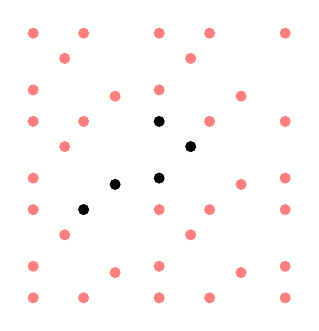
\begin{tikzpicture}[
    x = 0.8cm,
    y = 0.8cm,
    >=stealth,
    atom/.style = {circle, fill=black, minimum size=4pt,
    inner sep=0pt, outer sep=0pt},
    replica/.style = {circle, fill=red, minimum size=4pt,
    inner sep=0pt, outer sep=0pt, opacity=0.5},
]

    % \node[replica] (rep_0_00) at (0.0,0.0){};
    % \node[replica] (rep_1_00) at (0.5,0.4){};
    \node[replica] (rep_2_00) at (1.2,0.5){};
    \node[replica] (rep_3_00) at (1.2,1.4){};
    \node[replica] (rep_4_00) at (1.7,1.0){};
    % \draw [dashed] (0.0,0.0) -- (2.0,0.0);
    % \draw [dashed] (0.0,0.0) -- (0.0,1.4);
    % \node[replica] (rep_0_01) at (0.0,1.4){};
    % \node[replica] (rep_1_01) at (0.5,1.7999999999999998){};
    \node[replica] (rep_2_01) at (1.2,1.9){};
    \node[replica] (rep_3_01) at (1.2,2.8){};
    \node[replica] (rep_4_01) at (1.7,2.4){};
    % \draw [dashed] (0.0,1.4) -- (2.0,1.4);
    % \draw [dashed] (0.0,1.4) -- (0.0,2.8);
    % \node[replica] (rep_0_02) at (0.0,2.8){};
    % \node[replica] (rep_1_02) at (0.5,3.1999999999999997){};
    \node[replica] (rep_2_02) at (1.2,3.3){};
    \node[replica] (rep_3_02) at (1.2,4.199999999999999){};
    \node[replica] (rep_4_02) at (1.7,3.8){};
    % \draw [dashed] (0.0,2.8) -- (2.0,2.8);
    % \draw [dashed] (0.0,2.8) -- (0.0,4.199999999999999);
    \node[replica] (rep_0_10) at (2.0,0.0){};
    \node[replica] (rep_1_10) at (2.5,0.4){};
    \node[replica] (rep_2_10) at (3.2,0.5){};
    \node[replica] (rep_3_10) at (3.2,1.4){};
    \node[replica] (rep_4_10) at (3.7,1.0){};
    % \draw [dashed] (2.0,0.0) -- (4.0,0.0);
    % \draw [dashed] (2.0,0.0) -- (2.0,1.4);
    \node[atom] (atom_0) at (2.0,1.4){};
    \node[atom] (atom_1) at (2.5,1.7999999999999998){};
    \node[atom] (atom_2) at (3.2,1.9){};
    \node[atom] (atom_3) at (3.2,2.8){};
    \node[atom] (atom_4) at (3.7,2.4){};
    % \draw [dashed] (2.0,1.4) -- (4.0,1.4);
    % \draw [dashed] (2.0,1.4) -- (2.0,2.8);
    \node[replica] (rep_0_12) at (2.0,2.8){};
    \node[replica] (rep_1_12) at (2.5,3.1999999999999997){};
    \node[replica] (rep_2_12) at (3.2,3.3){};
    \node[replica] (rep_3_12) at (3.2,4.199999999999999){};
    \node[replica] (rep_4_12) at (3.7,3.8){};
    % \draw [dashed] (2.0,2.8) -- (4.0,2.8);
    % \draw [dashed] (2.0,2.8) -- (2.0,4.199999999999999);
    \node[replica] (rep_0_20) at (4.0,0.0){};
    \node[replica] (rep_1_20) at (4.5,0.4){};
    \node[replica] (rep_2_20) at (5.2,0.5){};
    \node[replica] (rep_3_20) at (5.2,1.4){};
    % \node[replica] (rep_4_20) at (5.7,1.0){};
    % \draw [dashed] (4.0,0.0) -- (6.0,0.0);
    % \draw [dashed] (4.0,0.0) -- (4.0,1.4);
    \node[replica] (rep_0_21) at (4.0,1.4){};
    \node[replica] (rep_1_21) at (4.5,1.7999999999999998){};
    \node[replica] (rep_2_21) at (5.2,1.9){};
    \node[replica] (rep_3_21) at (5.2,2.8){};
    % \node[replica] (rep_4_21) at (5.7,2.4){};
    % \draw [dashed] (4.0,1.4) -- (6.0,1.4);
    % \draw [dashed] (4.0,1.4) -- (4.0,2.8);
    \node[replica] (rep_0_22) at (4.0,2.8){};
    \node[replica] (rep_1_22) at (4.5,3.1999999999999997){};
    % \node[replica] (rep_2_22) at (5.2,3.3){};
    \node[replica] (rep_3_22) at (5.2,4.199999999999999){};
    % \node[replica] (rep_4_22) at (5.7,3.8){};
    % \draw [dashed] (4.0,2.8) -- (6.0,2.8);
    % \draw [dashed] (4.0,2.8) -- (4.0,4.199999999999999);
    % \draw [solid, very thick] (2.0,1.4) -- (4.0,1.4);
% \draw [solid, very thick] (4.0,1.4) -- (4.0,2.8);
% \draw [solid, very thick] (4.0,2.8) -- (2.0,2.8);
% \draw [solid, very thick] (2.0,2.8) -- (2.0,1.4);
% \draw [dashed] (6.0,0.0) -- (6.0,4.199999999999999);
% \draw [dashed] (6.0,4.199999999999999) -- (0.0,4.199999999999999);

% extral replicas sigh
% \node[replica] (rep_0_t02) at (0.0,4.2){};
\node[replica] (rep_0_t12) at (2.0,4.2){};
\node[replica] (rep_0_t22) at (4.0,4.2){};
% \node[replica] (rep_0_t32) at (6.0,4.2){};
% \node[replica] (rep_0_t31) at (6.0,2.8){};
% \node[replica] (rep_0_t30) at (6.0,1.4){};
% \node[replica] (rep_0_t30) at (6.0,00){};

\node[replica] (rep_3_b00) at (1.2,0.0){};
\node[replica] (rep_3_b10) at (3.2,0.0){};
\node[replica] (rep_3_b20) at (5.2,0.0){};


% \draw [solid, very thick] (rep_4_00) -- (atom_0);
% \draw [solid, very thick] (atom_0) -- (atom_1);
% \draw [solid, very thick] (atom_1) -- (atom_2);
% \draw [solid, very thick] (atom_2) -- (atom_4);
% \draw [solid, very thick] (atom_2) -- (rep_3_10);
% \draw [solid, very thick] (atom_3) -- (atom_4);
% \draw [solid, very thick] (atom_3) -- (rep_2_12);
% \draw [solid, very thick] (atom_4) -- (rep_0_22);

% \draw [solid, very thick] (rep_4_00) -- (rep_3_00);
% \draw [solid, very thick] (rep_4_00) -- (rep_2_00);

% \draw [solid, very thick] (rep_3_10) -- (rep_4_10);

% \draw [solid, very thick] (rep_0_22) -- (rep_1_22);

% \draw [solid, very thick] (rep_2_12) -- (rep_1_12);
% \draw [solid, very thick] (rep_2_12) -- (rep_4_12);

% \draw [solid, very thick] (rep_2_12) -- (rep_1_12);

% \draw [dotted, very thick] (rep_2_00) -- (rep_3_b00);
% \draw [dotted, very thick] (rep_2_01) -- (rep_3_00);
% \draw [dotted, very thick] (rep_2_01) -- (rep_4_01);

% \draw [dotted, very thick] (rep_2_02) -- (rep_3_01);
% \draw [dotted, very thick] (rep_2_02) -- (rep_4_02);

% \draw [dotted, very thick] (rep_3_02) -- (rep_4_02);
% \draw [dotted, very thick] (rep_4_02) -- (rep_0_t12);

% \draw [dotted, very thick] (rep_4_01) -- (rep_0_12);
% \draw [dotted, very thick] (rep_4_01) -- (rep_3_01);

% \draw [dotted, very thick] (rep_0_12) -- (rep_1_12);

% \draw [dotted, very thick] (rep_4_12) -- (rep_3_12);
% \draw [dotted, very thick] (rep_4_12) -- (rep_0_t22);

% \draw [dotted, very thick] (rep_0_10) -- (rep_1_10);
% \draw [dotted, very thick] (rep_1_10) -- (rep_2_10);
% \draw [dotted, very thick] (rep_2_10) -- (rep_3_b10);
% \draw [dotted, very thick] (rep_2_10) -- (rep_4_10);
% \draw [dotted, very thick] (rep_4_10) -- (rep_0_21);
% \draw [dotted, very thick] (rep_0_21) -- (rep_1_21);
% \draw [dotted, very thick] (rep_1_21) -- (rep_2_21);
% \draw [dotted, very thick] (rep_2_21) -- (rep_3_20);

% \draw [dotted, very thick] (rep_1_22) -- (rep_2_22);
% \draw [dotted, very thick] (rep_2_22) -- (rep_3_21);

% \draw [dotted, very thick] (rep_0_20) -- (rep_1_20);
% \draw [dotted, very thick] (rep_1_20) -- (rep_2_20);
% \draw [dotted, very thick] (rep_2_20) -- (rep_3_b20);

% \draw [solid, very thick] (0.55,-0.1) rectangle (5.45,4.3);


\end{tikzpicture}
};
    \node (c) at (2.4,1.25) {
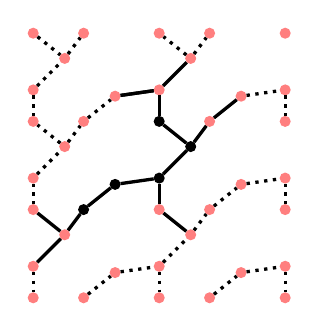
\begin{tikzpicture}[
    x = 0.8cm,
    y = 0.8cm,
    >=stealth,
    atom/.style = {circle, fill=black, minimum size=4pt,
    inner sep=0pt, outer sep=0pt},
    replica/.style = {circle, fill=red, minimum size=4pt,
    inner sep=0pt, outer sep=0pt, opacity=0.5},
]

    % \node[replica] (rep_0_00) at (0.0,0.0){};
    % \node[replica] (rep_1_00) at (0.5,0.4){};
    \node[replica] (rep_2_00) at (1.2,0.5){};
    \node[replica] (rep_3_00) at (1.2,1.4){};
    \node[replica] (rep_4_00) at (1.7,1.0){};
    % \draw [dashed] (0.0,0.0) -- (2.0,0.0);
    % \draw [dashed] (0.0,0.0) -- (0.0,1.4);
    % \node[replica] (rep_0_01) at (0.0,1.4){};
    % \node[replica] (rep_1_01) at (0.5,1.7999999999999998){};
    \node[replica] (rep_2_01) at (1.2,1.9){};
    \node[replica] (rep_3_01) at (1.2,2.8){};
    \node[replica] (rep_4_01) at (1.7,2.4){};
    % \draw [dashed] (0.0,1.4) -- (2.0,1.4);
    % \draw [dashed] (0.0,1.4) -- (0.0,2.8);
    % \node[replica] (rep_0_02) at (0.0,2.8){};
    % \node[replica] (rep_1_02) at (0.5,3.1999999999999997){};
    \node[replica] (rep_2_02) at (1.2,3.3){};
    \node[replica] (rep_3_02) at (1.2,4.199999999999999){};
    \node[replica] (rep_4_02) at (1.7,3.8){};
    % \draw [dashed] (0.0,2.8) -- (2.0,2.8);
    % \draw [dashed] (0.0,2.8) -- (0.0,4.199999999999999);
    \node[replica] (rep_0_10) at (2.0,0.0){};
    \node[replica] (rep_1_10) at (2.5,0.4){};
    \node[replica] (rep_2_10) at (3.2,0.5){};
    \node[replica] (rep_3_10) at (3.2,1.4){};
    \node[replica] (rep_4_10) at (3.7,1.0){};
    % \draw [dashed] (2.0,0.0) -- (4.0,0.0);
    % \draw [dashed] (2.0,0.0) -- (2.0,1.4);
    \node[atom] (atom_0) at (2.0,1.4){};
    \node[atom] (atom_1) at (2.5,1.7999999999999998){};
    \node[atom] (atom_2) at (3.2,1.9){};
    \node[atom] (atom_3) at (3.2,2.8){};
    \node[atom] (atom_4) at (3.7,2.4){};
    % \draw [dashed] (2.0,1.4) -- (4.0,1.4);
    % \draw [dashed] (2.0,1.4) -- (2.0,2.8);
    \node[replica] (rep_0_12) at (2.0,2.8){};
    \node[replica] (rep_1_12) at (2.5,3.1999999999999997){};
    \node[replica] (rep_2_12) at (3.2,3.3){};
    \node[replica] (rep_3_12) at (3.2,4.199999999999999){};
    \node[replica] (rep_4_12) at (3.7,3.8){};
    % \draw [dashed] (2.0,2.8) -- (4.0,2.8);
    % \draw [dashed] (2.0,2.8) -- (2.0,4.199999999999999);
    \node[replica] (rep_0_20) at (4.0,0.0){};
    \node[replica] (rep_1_20) at (4.5,0.4){};
    \node[replica] (rep_2_20) at (5.2,0.5){};
    \node[replica] (rep_3_20) at (5.2,1.4){};
    % \node[replica] (rep_4_20) at (5.7,1.0){};
    % \draw [dashed] (4.0,0.0) -- (6.0,0.0);
    % \draw [dashed] (4.0,0.0) -- (4.0,1.4);
    \node[replica] (rep_0_21) at (4.0,1.4){};
    \node[replica] (rep_1_21) at (4.5,1.7999999999999998){};
    \node[replica] (rep_2_21) at (5.2,1.9){};
    \node[replica] (rep_3_21) at (5.2,2.8){};
    % \node[replica] (rep_4_21) at (5.7,2.4){};
    % \draw [dashed] (4.0,1.4) -- (6.0,1.4);
    % \draw [dashed] (4.0,1.4) -- (4.0,2.8);
    \node[replica] (rep_0_22) at (4.0,2.8){};
    \node[replica] (rep_1_22) at (4.5,3.1999999999999997){};
    \node[replica] (rep_2_22) at (5.2,3.3){};
    \node[replica] (rep_3_22) at (5.2,4.199999999999999){};
    % \node[replica] (rep_4_22) at (5.7,3.8){};
    % \draw [dashed] (4.0,2.8) -- (6.0,2.8);
    % \draw [dashed] (4.0,2.8) -- (4.0,4.199999999999999);
    % \draw [solid, very thick] (2.0,1.4) -- (4.0,1.4);
% \draw [solid, very thick] (4.0,1.4) -- (4.0,2.8);
% \draw [solid, very thick] (4.0,2.8) -- (2.0,2.8);
% \draw [solid, very thick] (2.0,2.8) -- (2.0,1.4);
% \draw [dashed] (6.0,0.0) -- (6.0,4.199999999999999);
% \draw [dashed] (6.0,4.199999999999999) -- (0.0,4.199999999999999);

% extral replicas sigh
% \node[replica] (rep_0_t02) at (0.0,4.2){};
\node[replica] (rep_0_t12) at (2.0,4.2){};
\node[replica] (rep_0_t22) at (4.0,4.2){};
% \node[replica] (rep_0_t32) at (6.0,4.2){};
% \node[replica] (rep_0_t31) at (6.0,2.8){};
% \node[replica] (rep_0_t30) at (6.0,1.4){};
% \node[replica] (rep_0_t30) at (6.0,00){};

\node[replica] (rep_3_b00) at (1.2,0.0){};
\node[replica] (rep_3_b10) at (3.2,0.0){};
\node[replica] (rep_3_b20) at (5.2,0.0){};


\draw [solid, very thick] (rep_4_00) -- (atom_0);
\draw [solid, very thick] (atom_0) -- (atom_1);
\draw [solid, very thick] (atom_1) -- (atom_2);
\draw [solid, very thick] (atom_2) -- (atom_4);
\draw [solid, very thick] (atom_2) -- (rep_3_10);
\draw [solid, very thick] (atom_3) -- (atom_4);
\draw [solid, very thick] (atom_3) -- (rep_2_12);
\draw [solid, very thick] (atom_4) -- (rep_0_22);

\draw [solid, very thick] (rep_4_00) -- (rep_3_00);
\draw [solid, very thick] (rep_4_00) -- (rep_2_00);

\draw [solid, very thick] (rep_3_10) -- (rep_4_10);

\draw [solid, very thick] (rep_0_22) -- (rep_1_22);

\draw [solid, very thick] (rep_2_12) -- (rep_1_12);
\draw [solid, very thick] (rep_2_12) -- (rep_4_12);

\draw [solid, very thick] (rep_2_12) -- (rep_1_12);

\draw [dotted, very thick] (rep_2_00) -- (rep_3_b00);
\draw [dotted, very thick] (rep_2_01) -- (rep_3_00);
\draw [dotted, very thick] (rep_2_01) -- (rep_4_01);

\draw [dotted, very thick] (rep_2_02) -- (rep_3_01);
\draw [dotted, very thick] (rep_2_02) -- (rep_4_02);

\draw [dotted, very thick] (rep_3_02) -- (rep_4_02);
\draw [dotted, very thick] (rep_4_02) -- (rep_0_t12);

\draw [dotted, very thick] (rep_4_01) -- (rep_0_12);
\draw [dotted, very thick] (rep_4_01) -- (rep_3_01);

\draw [dotted, very thick] (rep_0_12) -- (rep_1_12);

\draw [dotted, very thick] (rep_4_12) -- (rep_3_12);
\draw [dotted, very thick] (rep_4_12) -- (rep_0_t22);

\draw [dotted, very thick] (rep_0_10) -- (rep_1_10);
\draw [dotted, very thick] (rep_1_10) -- (rep_2_10);
\draw [dotted, very thick] (rep_2_10) -- (rep_3_b10);
\draw [dotted, very thick] (rep_2_10) -- (rep_4_10);
\draw [dotted, very thick] (rep_4_10) -- (rep_0_21);
\draw [dotted, very thick] (rep_0_21) -- (rep_1_21);
\draw [dotted, very thick] (rep_1_21) -- (rep_2_21);
\draw [dotted, very thick] (rep_2_21) -- (rep_3_20);

\draw [dotted, very thick] (rep_1_22) -- (rep_2_22);
\draw [dotted, very thick] (rep_2_22) -- (rep_3_21);

\draw [dotted, very thick] (rep_0_20) -- (rep_1_20);
\draw [dotted, very thick] (rep_1_20) -- (rep_2_20);
\draw [dotted, very thick] (rep_2_20) -- (rep_3_b20);

% \draw [solid, very thick] (0.55,-0.1) rectangle (5.45,4.3);


\end{tikzpicture}
};
    \draw [->] (a) to node [midway, above]{Unfold} node [midway, below]{} (b) ;
    \draw [->] (b) to node [midway, above]{Construct} node [midway, below]{graph} (c) ;
  \end{tikzpicture}
  \caption{Construction of an \scare{unfolded} graph representation for the system in \cref{fig:glp-sketch_graph} with $\interactions{=}2$. First (left), $\Runf$ is determined by extending the simulation cell up to $\effcutoff$. Then (centre), positions in $\Runf$ are explicitly constructed. Finally (right), the input graph $\graph$ is constructed from all positions in $\Runf$. Positions in $\Rsc$ are marked in black, replicas in red. Edges that contribute to $U_i \in \Rsc$ are drawn as solid, others as dotted lines.}
  \label{fig:glp-fig_unf}
\end{figure*}

One solution, inspired by previous work on the derivation of the stress and heat flux for periodic systems~\cite{tpm2009t,khc2012t}, and illustrated in \cref{fig:glp-fig_unf}, lies in modifying the construction of $\graph$ to reflect the \scare{checkerboard} picture from \cref{ch:pbc}, constructing replicas explicitly. To this end, the simulation cell is extended, or \newterm{unfolded}, to include all positions that can interact with positions in the simulation cell. The graph is then construction for this unfolded simulation cell, $\Runf$, without the \mic. By construction, predictions for nodes representing atoms in $\Rsc$ are then identical, while derivatives of these potential energies $U_i$ with respect to positions in $\Runf$ distinguish between the simulation cell and replicas.

The unfolded simulation cell can be constructed efficiently by determining atoms that lie within $\effcutoff$ of the boundary; a brief overview over a practical implementation is given in \cref{sec:si-unf_imp}. The number of additional positions is proportional to the surface area of the simulation cell and therefore scales as $\bigo{N^{2/3}}$ (see \cref{sec:si-unfolding_n}). It is therefore asymptotically dominated by the increase in $N$ itself.


% For the quantities discussed in this section, this is unproblematic, but as will be discussed in \cref{ch:gk-hf}, this poses an essential difficulty for the computation of the heat flux, which requires the attribution of partial derivatives to replica positions.

% However, as we will see in \cref{ch:gk-hf}, this implicit treatment of periodicity introduces difficulties with the heat flux.


% \section{Local Potentials}

% \comm{TODO: Once the FF section is written, it should be referenced here.}
% The \glp framework also accommodates the \scare{bonded} terms of classical \ffs, as well as \mlps that are not explicitly defined as graph \nns, provided that atomic potential energies are computed based on atom-pair vectors, which is required by translational invariance.
% In particular, pair potentials can be seen a particular type of graph potential with $\interactions{=}1$, where $U_i$ is a direct sum over edge contributions,
% \begin{equation}
%     U_i = \sum_{j \in \nbh{i}} U_{ij}(|\R_{ij}|) \quad \text{with} \quad U_{ij} = U_{ji} \, . 
% \end{equation}
% The Lennard-Jones potential~\cite{l1924p} is a typical example, where
% \begin{align}
%     U_i &= 1/2 \sum_{j \in \nbh{i}} 4 \epsilon \left( \sigma^{12}/r_{ij}^{12} -\sigma^6/r_{ij}^6 \right) \, . \label{eq:glp_lj}
% \end{align}

% To illustrate this point, we briefly discuss pair potentials and the \scare{many-body} Tersoff potential~\cite{t1988p}.

% \paragraph{Pair Potentials} Pair potentials can be seen a particular type of graph potential with $\interactions=1$, where $U_i$ is a direct sum over edge contributions,
% \begin{align}
%     U_i &= \sum_{j \in \nbh{i}} U_{ij}(|\R_{ij}|) \label{eq:ui_pair} \\ 
%     U_{ij} &= U_{ji} \, . \label{eq:ui_pair_switch}
% \end{align}
% The Lennard-Jones potential~\cite{l1924p} is a typical example, where
% \begin{align}
%     U_i &= 1/2 \sum_{j \in \nbh{i}} 4 \epsilon \left( \sigma^{12}/r_{ij}^{12} -\sigma^6/r_{ij}^6 \right) \, . \label{eq:glp_lj}
% \end{align}

% \paragraph{Tersoff Potential} The Tersoff potential~\cite{t1988p} is a non-pairwise local potential. While it is also defined in terms of pairwise energies, these energies contain three-body information, rendering it a \scare{many-body} potential\footnote{While individual terms are composed of distance and angular terms, using two- and three-body information respectively, they are combined in a nonlinear fashion. Therefore, the potential cannot be separated into a sum over two- and three-body terms.} where $U_{ij} \neq U_{ji}$:
% \begin{align}
%     U_{ij} &= f_{\text{rep.}}(r_{ij}) - b_{ij} f_{\text{attr.}}(r_{ij}) \quad \neq U_{ji} \\
%     b_{ij} &= (1 + \beta^n \zeta_{ij}^n)^{-1/(2n)} \\
%     \zeta_{ij} &= \sum_{k \neq i,j} f_{\text{3-bdy}}(\R_{ij}, \R_{ik}) \, .
% \end{align}
% Here, $b_{ij}$ is a \newterm{bond-order} function, $f_{\text{rep.}}$ and $f_{\text{attr.}}$ a repulsive and attractive pair potential, and $f_{\text{3-bdy}}$ a function that takes the angle between $\R_{ij}$ and $\R_{ik}$ as well as $r_{ij}$ and $r_{ik}$ into account. Other variables are parameters that must be chosen empiricially for a given material.

% While this potential takes a more complex form, $U_i$ is nevertheless a pure function of edges within $\nbh{i}$, as pointed out by Fan~\etal~\cite{fpdh2015t}. The Tersoff potential can therefore be seen as a local \glp with $\interactions{=}1$.

% TODO: If we use Tersoff in the implementation paper, introduce Tersoff formula here. Otherwise, introduce Stilinger-Weber or similar.

\section{Derivatives}

As seen in \cref{ch:md}, the main quantities relevant for \md simulations are derivatives of the \pes. We now consider how to compute forces and stress using \ad.

\paragraph{Forces} For general \md simulations, we at least require the forces
\begin{equation}
    \F_i =-\dur{}{i}{} \, . \label{eq:glp_f_basic}
\end{equation}
Since $U$ is a scalar, and $\Rsc$ are an explicit input to its computation, the forces can be computed as a trivial \gls{jvp}\footnote{The product is over an output dimension of size \num{1}.} that can be evaluated with the same asymptotic cost as $U$.

An interesting situation arises if pairwise forces are desired. Strictly speaking, in a many-body potential, where interactions cannot be decomposed into pairwise contributions, such quantities are not well-defined and Newton's third law is replaced by conservation of momentum, which requires $\sum_{i=1}^N\nolimits \F_i = 0$. Nevertheless, pairwise forces with an antisymmetric structure can be defined by exploiting the construction of \glps{} in terms of atom-pair vectors.\footnote[][]{For pairwise distances, and without reference to graph structure, a more formal argument along similar lines appears in the work by Admal and Tadmor~\cite{at2011t}.}

$U$ is a function of all edges within $\interactions$ hops,
\begin{equation}
    U = U(\curlyset{\R_{ij}}{ij \in \edgest{i}}) \, .
\end{equation}
Hence, by the chain rule,
\begin{align}
    \F_i &= \sum_{j \in \nbh{i}} \dur{}{i}{j} - \dur{}{j}{i} \\
    &\defdas \sum_{j \in \nbh{i}} \F_{ij} \, .
\end{align}
\marginnote[-6\baselineskip]{In particular,
    \begin{equation}
        \dur{}{i}{} = \sum_{jk \in \edgest{i}} \dur{}{j}{k} \frac{\partial \R_{jk}}{\partial \R_i} \;,
    \end{equation}
    the second term is only non-vanishing when either $j$ or $k$ are $i$.
}
The pairwise forces such defined exhibit anti-symmetry, and therefore fulfil Newton's third law.
For $\interactions{=}1$, this recovers a more standard form~\cite{fpdh2015t} where only neighbouring atoms are involved,
\begin{equation}
    \F_{ij} = \dur{i}{i}{j} - \dur{j}{j}{i} \, .
\end{equation}
However, for $\interactions{>}1$, this calculation of pairwise forces includes a sum over all $U_k$ that are influenced by a given edge
\begin{equation}
    \F_{ij} = \sum_{k \in \nbht{i}} \dur{k}{i}{j} - \dur{k}{j}{i} \, ,
\end{equation}
subverting expectations connecting local potential energies to pairwise forces.
This apparent contradiction is a consequence of the combination of the peculiar construction of \glps and \ad: In principle, it is always possible to define extended neighbourhoods up to $\effcutoff$, obtaining $U_i$ purely as a function of atom-pair vectors originating from $i$.
However, to construct derivatives with respect to these atom-pair vectors with \ad, these extended neighbourhoods have to be computed explicitly, therefore negating the computational efficiency gains of a \glp architecture.

\paragraph{Stress} The definition of the (potential) stress is~\cite{kcbs2015t}
% \begin{equation}
%   \stressc^{\lambda \mu} = \frac{1}{V} \, \frac{\partial U'}{\partial \epsilon^{\lambda \mu}}{\big |}_{\epsilon = 0} \, ,
% \end{equation}
\begin{equation}
    \stress = \frac{1}{V} \, \frac{\partial U'}{\partial \strain}{\big |}_{\strain = 0} \, , \label{eq:glp_stress_gen}
\end{equation}
% with $U'$ denoting the potential energy after a strain transformation with the strain tensor $\strainc^{\lambda\mu}$, which transforms all positions as:
with $U'$ denoting the potential energy after a transformation of all positions with the $3\times3$ symmetric strain tensor $\strain$
\begin{equation}
    \R \rightarrow (\matone + \strain) \cdot \R \quad \text{for} \quad \R \in \Rall \, .
\end{equation}
While computing the derivative in \cref{eq:glp_stress_gen} for arbitrary potentials and periodic systems has been classified as requiring \scare{much effort}~\cite{lb2006p} in the past, and has been the focus of much discussion~\cite{tpm2009t,at2011t}, it is straightforward with \ad.

Two approaches are possible: \emph{(a)} \Cref{eq:glp_stress_gen} can be implemented directly by explicitly performing the strain transformation during the calculation of $U$, obtaining the stress with \ad by differentiating with respect to $\strain$, or \emph{(b)} \cref{eq:glp_stress_gen} can be re-written in terms of other derivatives, which are then computed with \ad.

\clearpage
This yields a number of equivalent definitions of the stress
% \marginnote{The notation $\symset{S}\rightarrow(\matone + \strain) \cdot \symset{S}$ indicates that $\strain$ is applied to all vectors in $\symset{S}$.}
\marginnote{The notation $\symset{S}'$ indicates that $\strain$ is applied to all vectors in $\symset{S}$.}
\marginnote{It must be stressed that the equivalence of the given formulations rests on definitions so far. For instance, the edges in $\graph$ must be constructed with the \mic as defined in \cref{eq:pbc_mic}. If they are instead computed using the modulo operation in fractional coordinates, the stress cannot be obtained directly from $\Rsc$ and $\Basis$; \cref{eq:glp_stress_strain_direct,eq:glp_stress_sc_basis} yield incorrect results.}
\marginnote{\Cref{eq:glp_stress_bulk} uses $\Runf$, the \scare{unfolded} simulation cell that contains all positions that contribute to atomic energies in the simulation cell. We defined it previously in \cref{sec:glp-unf}.}
\begin{align}
    V \stress 
    % &=\frac{\partial U(\Rsc\rightarrow(\matone + \strain) \cdot \Rsc, \Basis\rightarrow(\matone + \strain) \cdot \Basis)}{\partial \strain} \label{eq:glp_stress_strain_direct}\\
    % &=\frac{\partial U(\edges\rightarrow(\matone + \strain) \cdot \edges)}{\partial \strain} \label{eq:glp_stress_strain_edges}\\
    &=\frac{\partial U(\Rsc',\Basis')}{\partial \strain} \label{eq:glp_stress_strain_direct}\\
    &=\frac{\partial U(\edges')}{\partial \strain} \label{eq:glp_stress_strain_edges}\\
    &=\frac{\partial U(\Runf')}{\partial \strain} \label{eq:glp_stress_strain_unf}\\
    &=\sum_{i \in \Rsc} \R_j \otimes \dur{}{i}{} + \sum_{\basis \in \Basis} \basis \otimes \frac{\partial U}{\partial \basis} \label{eq:glp_stress_sc_basis}\\
    &= \sum_{ij \in \edges} \R_{ij} \otimes \dur{}{i}{j} \label{eq:glp_stress_edges}\\
    &= \sum_{i \in \Runf} \R_{i} \otimes \dur{}{i}{} \label{eq:glp_stress_bulk} \, .
\end{align}
recovering formulations given by Louwerse and Baerends~\cite{lb2006p} and Thompson~\cite{tpm2009t}.\footnote[][-2\baselineskip]{In particular, \cref{eq:glp_stress_sc_basis} appears as equation 8 in reference \cite{lb2006p} and \cref{eq:glp_stress_bulk} can be identified with equation 13 therein. \Cref{eq:glp_stress_sc_basis} is the \scare{atom-cell} form given in reference \cite[eq.~27]{tpm2009t}, \cref{eq:glp_stress_bulk} the \scare{atom} form in equation 25. In the case of pair-additive \glps with $\interactions{=}1$, \cref{eq:glp_stress_edges} reduces to the standard form which can be found, for example, in reference \cite[eq.~2]{lb2006p}.
}\footnote{
    Different forms are implemented in available \mlp packages. For example, \schnetpack~\cite{sktm2019q,schnetpack} and \nequip~\cite{bmsk2022q,nequip} implement \cref{eq:glp_stress_strain_direct}, \gls{mace} in \software{pytorch}~\cite{mace-torch} implements \cref{eq:glp_stress_strain_direct}, while \gls{mace} in \software{jax}~\cite{mace-jax} uses \cref{eq:glp_stress_sc_basis}.
} All formulations are compared in \cref{tab:glps_lj_stress_error_32} for the Lennard-Jones potential and in \cref{tab:glps_snse_stress_error_32} for the \sok~\cite{fum2022q} \glp with $\interactions{=}2$. They are found to be equivalent. Further discussion and details on these experiments can be found in \cref{sec:si-glp_testing} as well as reference~\cite{lfk2023a}.

\newthought{A more complex situation} arises if strain derivatives of atomic energies, in other words, atomic stresses
\begin{equation}
    V \stress_i \defas \frac{\partial U_i}{\partial \strain} \quad \text{for} \quad i \in \Rsc
\end{equation}
are required.
Their calculation requires either one backwards pass per $U_i$, or one forward pass for each entry in $\strain$. If only reverse-mode \ad is available, its evaluation therefore scales quadratically with $N$.  Linear scaling is retained with forward mode. 
For \glps with $\interactions{=}1$, linear scaling in reverse mode can be recovered by using \cref{eq:glp_stress_edges}: Every edge can be uniquely assigned to one $U_i$, and therefore the derivatives can be used to construct atomic stresses. For $\interactions{>}1$, this is not possible; similar to the observations for pairwise forces, atomic stresses take a semi-local form.

As will be discussed in \cref{ch:gk-hf}, similar issues arise in the calculation of the heat flux, which relies on derivatives of atomic potential energies $U_i$: A direct implementation requires separate \ad passes for each $U_i$ and leads to quadratic scaling.

\newthought{To summarise, this section} has introduced an abstract description of interatomic potentials in terms of a mapping between a graph $\graph$ of atom-pair vectors (the edges $\edges$) and atoms (the vertices $\vertices$) and a set of atomic potential energies $U_i$. In this framework, (pairwise) forces and the stress tensor can be defined and implemented in a unified way, not requiring further information about the structure of the potential. To illustrate this, and enable subsequent work, the \glpc package, using \jax~\cite{jax}, briefly discussed in \cref{sec:si-glp}, has been developed.

\begin{table}
    \caption[][-1\baselineskip]{
    Error in stress for Lennard-Jones argon,
    comparing different formulations, as well as finite differences, with an analytical implementation in \gls{ase}.
    % , where derivatives are obtained analytically.
    Results are shown for single precision arithmetic, and for $\stress \cdot V$ in place of $\stress$.
    }
    \begin{tabular}{l | r r r r}
\toprule
            Equation  &  \acs{mae} in \unit{eV}  &  \acs{maxae} in \unit{eV}  &  \acs{mape} in \unit{\percent}  &  \acs{maxape} in \unit{\percent} \\ 
\midrule
          Fin. diff.  &        \num{7.70e-04}  &        \num{4.18e-03}  &        \num{1.04e-01}  &        \num{5.30e+00} \\ 
\ref{eq:glp_stress_strain_direct}  &        \num{1.19e-05}  &        \num{6.54e-05}  &        \num{1.79e-03}  &        \num{7.35e-02} \\ 
\ref{eq:glp_stress_strain_edges}  &        \num{8.25e-06}  &        \num{4.11e-05}  &        \num{1.27e-03}  &        \num{6.75e-02} \\ 
\ref{eq:glp_stress_strain_unf}  &        \num{9.17e-06}  &        \num{4.46e-05}  &        \num{1.36e-03}  &        \num{4.39e-02} \\ 
\ref{eq:glp_stress_sc_basis}  &        \num{1.18e-05}  &        \num{6.44e-05}  &        \num{1.79e-03}  &        \num{7.19e-02} \\ 
\ref{eq:glp_stress_edges}  &        \num{8.22e-06}  &        \num{4.16e-05}  &        \num{1.27e-03}  &        \num{6.59e-02} \\ 
\ref{eq:glp_stress_bulk}  &        \num{9.16e-06}  &        \num{4.51e-05}  &        \num{1.37e-03}  &        \num{4.92e-02} \\ 
\bottomrule
\end{tabular}

    \label{tab:glps_lj_stress_error_32}
\end{table}

\begin{table}
    \caption[][-1\baselineskip]{
    Error in stress for \ch{SnSe}, using the $\interactions{=}2$ \sok model discussed further in \cref{ch:gk-out},
    comparing different formulations of the stress with finite differences.
    % , where derivatives are obtained analytically.
    Results are shown for single precision arithmetic, and for $\stress \cdot V$ in place of $\stress$.
    }
    \begin{tabular}{l | r r r r}
\toprule
            Equation  &  \acs{mae} in \unit{eV}  &  \acs{maxae} in \unit{eV}  &  \acs{mape} in \unit{\percent}  &  \acs{maxape} in \unit{\percent} \\ 
\midrule
\ref{eq:glp_stress_strain_direct}  &        \num{1.58e-02}  &        \num{8.26e-02}  &        \num{4.40e-02}  &        \num{7.01e-01} \\ 
\ref{eq:glp_stress_strain_edges}  &        \num{1.58e-02}  &        \num{8.26e-02}  &        \num{4.38e-02}  &        \num{6.92e-01} \\ 
\ref{eq:glp_stress_strain_unf}  &        \num{1.57e-02}  &        \num{8.37e-02}  &        \num{4.33e-02}  &        \num{6.69e-01} \\ 
\ref{eq:glp_stress_sc_basis}  &        \num{1.58e-02}  &        \num{8.27e-02}  &        \num{4.40e-02}  &        \num{7.00e-01} \\ 
\ref{eq:glp_stress_edges}  &        \num{1.58e-02}  &        \num{8.26e-02}  &        \num{4.38e-02}  &        \num{6.91e-01} \\ 
\ref{eq:glp_stress_bulk}  &        \num{1.57e-02}  &        \num{8.37e-02}  &        \num{4.33e-02}  &        \num{6.71e-01} \\ 
\bottomrule
\end{tabular}

    \label{tab:glps_snse_stress_error_32}
\end{table}
